\documentclass[journal]{IEEEtran}

\usepackage[utf8]{inputenc}
\usepackage[T1]{fontenc}
\usepackage[spanish,es-tabla,es-noquoting,es-nodecimaldot]{babel}
\usepackage{graphicx}
\usepackage{booktabs}
\usepackage{array}
\usepackage{tabularx}
\usepackage{amsmath}
\usepackage{url}

\newcolumntype{L}{>{\raggedright\arraybackslash}X}

\begin{document}

\title{Modelo predictivo de riesgo de mora en contratos de leasing de motocicletas\\
\large Proyecto de aula, Modelos y Simulación de Sistemas II: Entregable I}

\author{Juan Esteban Cardozo Rivera, Maria Carolina Cardona Calderon y Oliver Andres Quiroz Mora%
\thanks{Departamento de Ingeniería de Sistemas, Universidad de Antioquia, Colombia. Grupo 14.}}

\maketitle

% =====================================================================
\section{Descripción del problema}

\subsection{Contexto del problema}
\label{sec:contexto}

Una empresa de leasing de motocicletas con operación en Cartagena, Sincelejo y Montería, y con varios miles de contratos, otorga vehículos mediante pagos semanales o quincenales. Cuando un cliente paga después de la fecha esperada, se genera una multa que crece con los días de atraso y, en los casos de mal comportamiento de pago, la empresa puede retener el vehículo. Esta situación afecta el flujo de caja y hace costosa la gestión de cartera, que hoy se realiza de forma homogénea y reactiva, es decir, cuando el atraso ya ocurrió y sin distinguir entre clientes.

El proyecto busca resolver dos preguntas: (1) qué perfiles de comportamiento de pago existen en la cartera, lo cual se aborda con aprendizaje no supervisado al no existir una clasificación previa de los clientes; y (2) cuál es la probabilidad de que un contrato termine en riesgo grave de mora, lo cual se aborda con aprendizaje supervisado, usando como entrada las variables del historial de pagos de las primeras semanas del contrato y el perfil identificado en la primera etapa. Con ello se pretende que el área de cartera pueda ordenar los contratos por nivel de riesgo y priorizar los esfuerzos de cobranza desde etapas tempranas.

Para el desarrollo de este proyecto, el análisis se delimita a los datos de la sede Cartagena, debido a que es la sede más grande y significativa de la empresa en términos de operación y volumen de contratos (3.906 contratos y 5.316 episodios de leasing en la base analizada). Esta delimitación permite concentrar el estudio en una cartera con suficiente cantidad y diversidad de registros para identificar patrones de comportamiento de pago y construir modelos de predicción de riesgo. Además, trabajar con una única sede permite reducir posibles diferencias asociadas a las características particulares de cada zona y establecer un alcance controlado para el desarrollo y evaluación de la metodología propuesta.

\subsection{Objetivo general}

Diseñar, entrenar y evaluar un sistema de aprendizaje de máquina en dos etapas que (1) identifique perfiles de comportamiento de pago en la cartera de contratos de leasing de motocicletas mediante aprendizaje no supervisado y (2) estime, mediante aprendizaje supervisado, la probabilidad de que un contrato termine en riesgo grave de mora a partir del historial de pagos de las primeras semanas y del perfil identificado, con el fin de apoyar la priorización temprana de la gestión de cobranza.

\subsection{Objetivos específicos}

\begin{itemize}
\item Caracterizar la base de datos real y documentar su estructura, variables, calidad y restricciones.
\item Definir formalmente la variable objetivo ``riesgo grave de mora'', el horizonte temporal de predicción y el número de semanas iniciales usadas como entrada, evitando fuga de información.
\item Construir un flujo reproducible de limpieza, codificación, ingeniería de variables y escalamiento.
\item Identificar perfiles de comportamiento de pago mediante técnicas de aprendizaje no supervisado y caracterizarlos.
\item Entrenar y comparar al menos cinco modelos supervisados de clasificación para estimar la probabilidad de riesgo grave de mora.
\item Evaluar el aporte del perfil (etapa 1) como variable de entrada de la etapa 2.
\item Evaluar el efecto de la selección y reducción de variables mediante análisis individual de variables, PCA y UMAP.
\item Comparar desempeño, complejidad e interpretabilidad para seleccionar la solución final y proponer su uso para ordenar contratos por riesgo.
\item Documentar las limitaciones, los riesgos de uso y las condiciones necesarias para una implementación responsable.
\end{itemize}

\subsection{Preguntas de investigación}

El proyecto busca resolver dos preguntas, cada una asociada a un paradigma de aprendizaje distinto:
\begin{itemize}
\item Pregunta 1 (aprendizaje no supervisado): ¿qué perfiles de comportamiento de pago existen en la cartera? Al no existir una clasificación previa de los clientes, el problema se aborda sin etiquetas.
\item Pregunta 2 (aprendizaje supervisado): ¿cuál es la probabilidad de que un contrato termine en riesgo grave de mora, usando como entrada las variables del historial de pagos de las primeras semanas del contrato y el perfil identificado en la primera etapa?
\end{itemize}

% ---------------------------------------------------------------------
\subsection{Composición de la base de datos}

La base proviene del sistema operativo de la empresa (MySQL) y corresponde a la sede Cartagena. Se usaron tres tablas, resumidas en la Tabla~\ref{tab:fuentes}, de las que se extrajeron solo las columnas necesarias y se reemplazó el número de contrato por un código anónimo. Antes del análisis se excluyeron los registros fuera de alcance: los de la empresa RastreoYa (4.475 registros, cuyos identificadores eran correos electrónicos), los contratos no numéricos y 15 contratos de ventas a Medellín.

\begin{table}[!t]
\caption{Fuentes de datos}
\label{tab:fuentes}
\centering
\small
\begin{tabularx}{\columnwidth}{@{}lLr@{}}
\toprule
Tabla & Contenido & Registros \\
\midrule
Historial de abonos & Un registro por contrato y fecha de pago (2020-02-09 a 2026-10-03) & 214.745 \\
Foto diaria & Estado de cada moto por día desde 2024-03-30: inicio, frecuencia, cuota y justificaciones & 1.260.006 \\
Rentabilidad & Episodios cerrados con su desenlace & 3.531 \\
\bottomrule
\end{tabularx}
\end{table}

El hallazgo central de la exploración es que el número de contrato identifica la motocicleta y no al cliente: cuando a un cliente se le retira la moto, esta se asigna a otro con el mismo número. De los 3.081 contratos de la foto diaria, 1.732 tienen dos o más fechas de inicio. Por eso la unidad de análisis es el \emph{episodio}, es decir, un cliente con una moto, identificado por el contrato y su fecha de inicio. En adelante, cuando se habla del riesgo de un contrato, se refiere al episodio vigente de ese contrato. La base tiene 3.906 contratos y 5.316 episodios de leasing (4.371 semanales y 135 quincenales desde 2024-03-30). La muestra para modelar tiene 2.933 episodios, cada uno descrito por 24 variables candidatas (19 de comportamiento de pago y 5 del contrato) y la etiqueta. La Tabla~\ref{tab:columnas} resume las columnas usadas y su significado de negocio; los montos están en miles de pesos.

\begin{table}[!t]
\caption{Columnas usadas y significado de negocio}
\label{tab:columnas}
\centering
\small
\begin{tabularx}{\columnwidth}{@{}lL@{}}
\toprule
Columna & Significado \\
\midrule
Fecha & Fecha del registro de pago \\
Abono, transferencia & Pago al canon; lo único que reduce el saldo de la moto \\
Multa & Multa por atraso cobrada en el pago \\
Repuesto & Devolución de dinero prestado al cliente (repuestos, trámites, SOAT) \\
Carta y motivo & Abono ficticio que cierra el saldo cuando la moto deja de estar con el cliente, y su motivo \\
Fecha de inicio & Inicio del episodio \\
Tipo de pago, día de canon & Frecuencia de pago y día de vencimiento de la cuota \\
Cuota, cuotas pactadas & Valor de la cuota y duración pactada \\
Justificación & Justificación del cliente o marca de gestión vigente ese día \\
Empresa & Empresa del grupo (MotoHoy o RentaYa) \\
\bottomrule
\end{tabularx}
\end{table}

Los faltantes del motivo de carta y de la justificación son estructurales: solo se llenan cuando hay carta o justificación. Los faltantes reales encontrados fueron: 1.692 tramos con fecha de inicio 0000-00-00, que corresponden a clientes asignados con trámites pendientes, todavía sin la moto; 18 episodios semanales sin día de vencimiento, para los que no se puede construir el calendario de pagos; 39.760 registros con el código 999 en los días sin pagar, que el sistema usa cuando aún no hay pagos; y la multa en 0 en todos los pagos de 2020 a 2022, porque no se registraba en ese período, lo que no equivale a ``sin multa''. La estrategia de imputación se detalla en la Sección~\ref{sec:calidad}. Las variables categóricas se codifican así: frecuencia de pago y empresa como binarias, y día de vencimiento (martes, miércoles, jueves o quincenal) con codificación one-hot. Las numéricas se estandarizan dentro del flujo de entrenamiento.

% ---------------------------------------------------------------------
\subsection{Definición de la variable objetivo y prevención de fuga de información}

\textbf{Fecha esperada de pago.} La base no registra la fecha esperada de cada pago, por lo que se reconstruye el calendario de cada episodio. Para pago semanal, la cuota vence cada día de canon a partir de la fecha de inicio; para pago quincenal, cada 14 días. El 48~\% de los pagos semanales cae exactamente el día de canon (Fig.~\ref{fig:canon}), y la multa aparece desde el día siguiente: el 96,2~\% de las cuotas pagadas a tiempo no tiene multa, mientras que el 83,1~\% de las pagadas con uno o dos días de atraso sí la tiene. Para la empresa hubo pago si el cliente entregó cualquier dinero ese día, aunque se descuente a multa o repuesto; el mal comportamiento es no entregar nada. Cada día con pago cubre una cuota del calendario, o varias si el monto alcanza varias cuotas, y el atraso de una cuota es la diferencia entre la fecha del pago que la cubrió y su fecha de vencimiento.

\begin{figure}[!t]
\centering
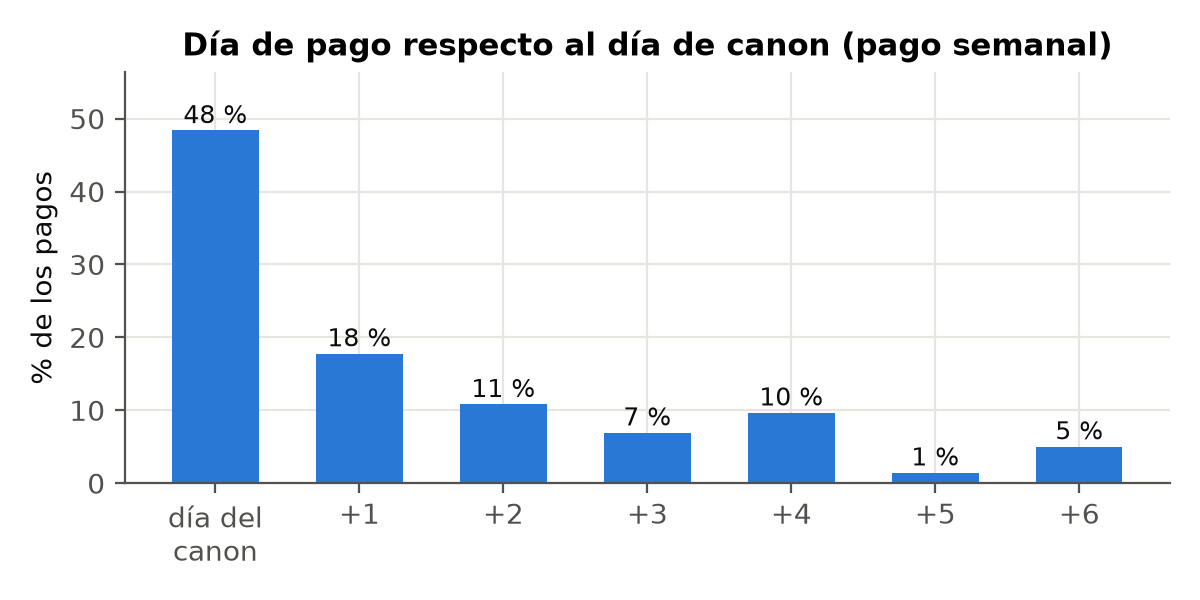
\includegraphics[width=\columnwidth]{figuras/dia_pago_vs_canon.png}
\caption{Día de pago respecto al día de canon en contratos semanales (pagos desde 2024).}
\label{fig:canon}
\end{figure}

\textbf{Evento objetivo.} Un episodio está en riesgo grave de mora si alguna cuota que vence en la ventana de predicción alcanza 14 o más días de atraso, lo que equivale a dos cuotas semanales sin pagar. También cuenta como evento la cuota que nunca se pagó porque el episodio se cerró antes de llegar a 14 días. El umbral se eligió con la distribución real del atraso (Fig.~\ref{fig:umbral}): al comparar el máximo atraso de una cuota en la ventana con el porcentaje de episodios que terminan con la moto retirada, el retiro pasa del 13--16~\% sin atraso relevante al 47~\% con 7 a 13 días, y se estabiliza en 66--72~\% desde los 14 días. Desde ese punto, más días de atraso ya no aumentan el riesgo.

\begin{figure}[!t]
\centering
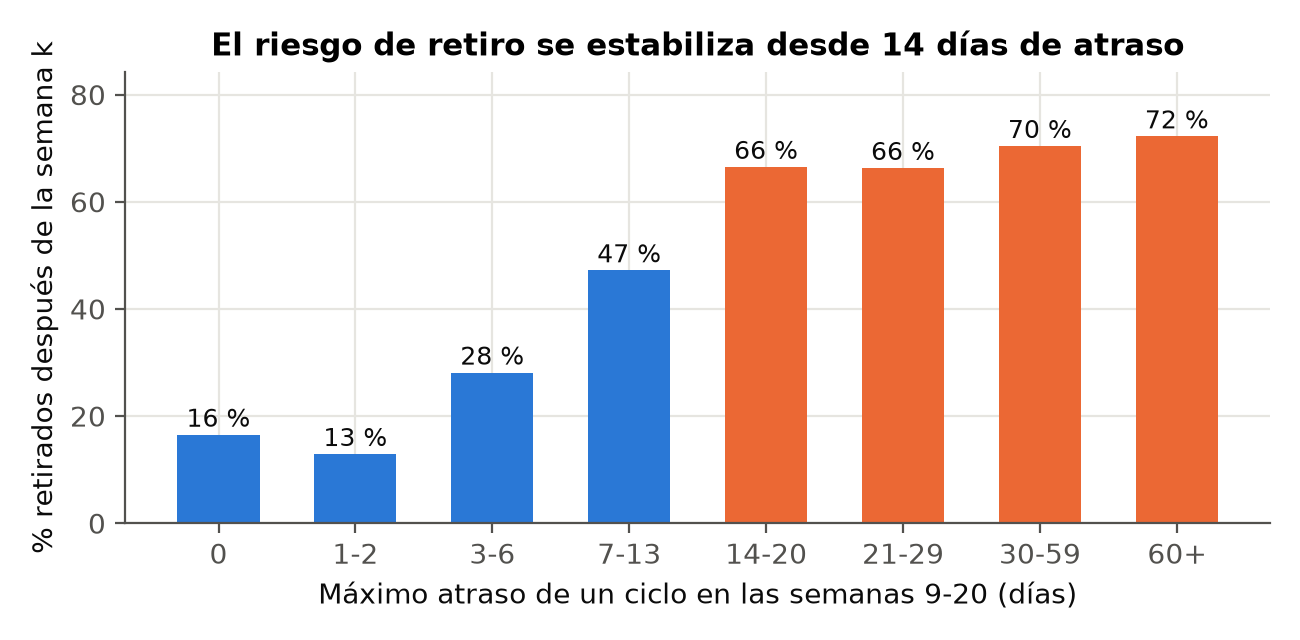
\includegraphics[width=\columnwidth]{figuras/retiro_vs_atraso_maximo.png}
\caption{Porcentaje de episodios retirados según el máximo atraso de una cuota en la ventana de predicción ($k=8$, $H=12$).}
\label{fig:umbral}
\end{figure}

\textbf{Ventanas y fecha de corte.} Para cada episodio, la fecha de corte es $t_k$ = fecha de inicio + $k$ semanas, con $k=8$. La ventana de observación son las semanas 1 a 8 del episodio: las variables de entrada solo usan información con fecha anterior o igual a $t_k$, y una cuota vencida antes de $t_k$ y pagada después se registra como no pagada, con el atraso acumulado hasta $t_k$, porque es lo que se sabría ese día. La ventana de predicción son las semanas 9 a 20 ($H=12$ semanas). Se eligió $k=8$ porque ofrece ocho cuotas semanales (cuatro quincenales), suficientes para medir regularidad y variabilidad; con $k=4$ solo habría cuatro cuotas, y con $k=12$ se perderían 960 episodios retirados antes de poder predecir. El horizonte de 12 semanas coincide con el de mejor desempeño reportado en [3] y conserva episodios de 2026.

\textbf{Regla de etiquetado.} $y=1$ si alguna cuota con vencimiento en las semanas 9 a 20 alcanza 14 o más días de atraso, o nunca se pagó porque el episodio se cerró; $y=0$ en cualquier otro caso.

\textbf{Población.} Entran los episodios que iniciaron desde el 2024-03-30, fecha en que empieza la foto diaria; los episodios anteriores solo aparecen si seguían activos ese día, lo que sesgaría la muestra hacia clientes que sobrevivieron. Además, el episodio debe seguir con la moto en $t_k$ y su desenlace debe ser observable antes del corte de datos (2026-10-03). Se excluyeron 810 episodios anteriores a la cohorte, 225 errores de asignación (una semana o menos sin ningún pago), 18 sin día de vencimiento, 994 cerrados antes de la semana 8 y 336 recientes sin desenlace observable todavía.

El retiro del vehículo y las marcas de gestión de la empresa no forman parte de la etiqueta, porque son decisiones discrecionales sin una regla fija; el retiro solo se usa para validar el umbral. De los 1.070 episodios positivos, 766 lo son por atraso de 14 o más días y 304 por una cuota nunca pagada; de estos, 260 terminaron con la moto retirada en promedio siete días después de la cuota incumplida, antes de llegar al umbral.

% ---------------------------------------------------------------------
\subsection{Variables candidatas confirmadas en la base real}

La Tabla~\ref{tab:variables} lista las variables candidatas. Todas se calculan con las primeras 8 semanas de cada episodio y se expresan como proporciones o promedios por cuota, para que sean comparables entre pago semanal y quincenal. La última columna es la correlación de Spearman con la etiqueta (Fig.~\ref{fig:spearman}).

\begin{table*}[!t]
\caption{Variables candidatas de las primeras 8 semanas}
\label{tab:variables}
\centering
\small
\begin{tabularx}{\textwidth}{@{}llLr@{}}
\toprule
Variable & Fuente & Definición & $\rho$ \\
\midrule
Proporción de cuotas atrasadas & Abonos y calendario & Cuotas con 1 o más días de atraso / cuotas vencidas & 0,43 \\
Proporción de cuotas con atraso de 3 o más días & Abonos y calendario & Cuotas con 3 o más días de atraso / cuotas vencidas & 0,46 \\
Atraso promedio & Abonos y calendario & Días de atraso promedio por cuota & 0,47 \\
Atraso máximo & Abonos y calendario & Mayor atraso de una cuota & 0,48 \\
Cuotas sin pagar en $t_k$ & Abonos y calendario & Cuotas vencidas sin pago al momento de predecir & 0,47 \\
Pagos por cuota & Abonos & Días con pago / cuotas vencidas & $-0{,}44$ \\
Déficit relativo & Abonos y foto diaria & $1 - (\text{abono} + \text{transferencia}) / (\text{cuota} \times \text{cuotas vencidas})$ & 0,44 \\
Variabilidad del abono & Abonos & Coeficiente de variación del pago al canon & 0,15 \\
Multa acumulada & Abonos & Suma de multas & 0,23 \\
Proporción de pagos con multa & Abonos & Pagos con multa / pagos & 0,30 \\
Repuesto acumulado & Abonos & Dinero devuelto por préstamos & 0,09 \\
Días hasta el primer pago & Abonos & Días entre el inicio y el primer pago & 0,03 \\
Justificaciones por enfermedad & Foto diaria & Eventos de enfermedad o calamidad familiar & 0,08 \\
Justificaciones por inmovilización & Foto diaria & Eventos de moto varada, accidentada, en patio, en taller, en garantía o en Fiscalía & 0,13 \\
Retención temporal & Foto diaria & Eventos de moto ingresada (la empresa la retiene alrededor de una semana) & 0,15 \\
Cliente problema & Foto diaria & Eventos de cliente marcado como problema & $-0{,}01$ \\
Frecuencia de pago & Foto diaria & Semanal o quincenal & -- \\
Empresa & Foto diaria & MotoHoy o RentaYa & -- \\
Cuota & Foto diaria & Valor de la cuota & $-0{,}02$ \\
Cuotas pactadas & Foto diaria & Duración pactada del contrato & 0,00 \\
Día de vencimiento & Foto diaria & Martes, miércoles, jueves o quincenal & -- \\
\bottomrule
\end{tabularx}
\end{table*}

\begin{figure}[!t]
\centering
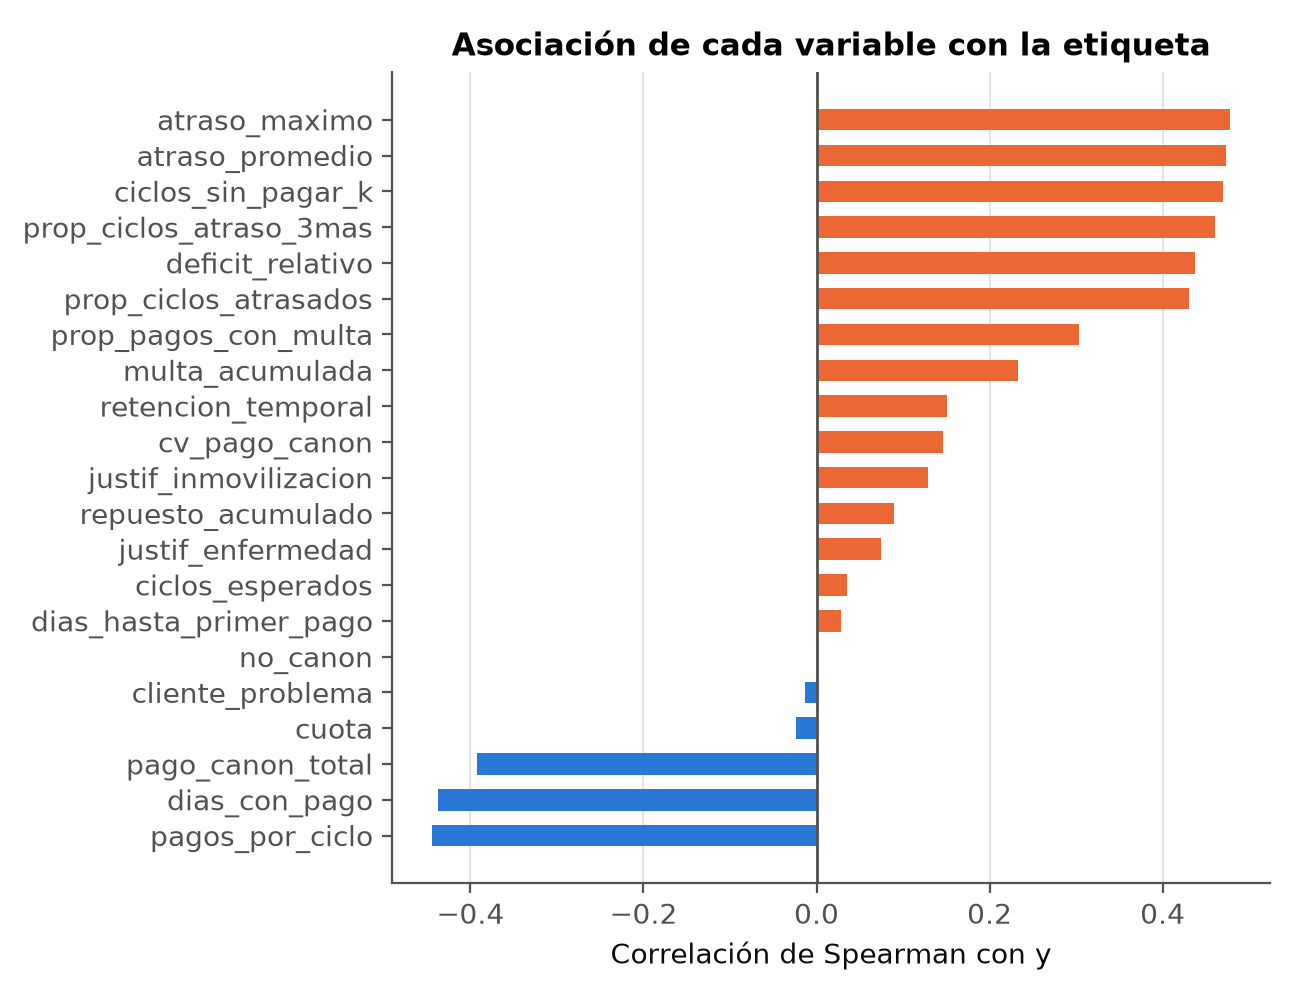
\includegraphics[width=\columnwidth]{figuras/spearman_variables.png}
\caption{Correlación de Spearman de cada variable candidata con la etiqueta.}
\label{fig:spearman}
\end{figure}

Tres variables del caso no se confirmaron como se habían planteado. La ciudad no se incluye porque el estudio se limita a la sede Cartagena (Sección~\ref{sec:contexto}). Las semanas observadas son iguales a 8 para todos los episodios de la población, así que no aportan información; su equivalente por frecuencia es el número de cuotas vencidas. La frecuencia de pago está vacía en el 70~\% de los registros del historial de abonos, por lo que se toma de la foto diaria.

La retención temporal y el cliente problema son marcas de gestión de la empresa, no comportamientos del cliente. Se conocen al momento de predecir y no producen fuga de información, pero el modelo se evaluará con y sin ellas para no aprender solo las decisiones de cartera. La prevalencia de la etiqueta también varía por empresa (31,1~\% en MotoHoy y 55,6~\% en RentaYa), lo que respalda incluir la empresa como variable.

% ---------------------------------------------------------------------
\subsection{Calidad y preparación de datos}
\label{sec:calidad}

\textbf{Consistencia de la multa.} La multa se cobra por escalones según el atraso dentro de la semana: sin multa al día, 15 mil con uno o dos días de atraso y 25 mil desde tres días. La correlación de Spearman entre multa y días de atraso por cuota es 0,61. La relación se debilita desde siete días porque un cliente que va una semana atrasado pero paga el día de canon muchas veces no recibe multa. La proporción de pagos con multa es casi redundante con la proporción de cuotas atrasadas ($\rho=0{,}84$), y también son redundantes los pares atraso máximo y promedio ($\rho=0{,}97$) y pagos por cuota y días con pago ($\rho=0{,}99$). Estos pares se resolverán con el análisis individual de variables y la reducción de dimensión del Entregable II.

\textbf{Estrategia de imputación.} Ningún faltante se reemplaza por un valor inventado sin dejar rastro (Tabla~\ref{tab:imputacion}). Cualquier imputación que dependa de estadísticos de los datos se ajusta solo con el conjunto de entrenamiento, dentro de cada pliegue de validación.

\begin{table*}[!t]
\caption{Diagnóstico de faltantes y estrategia de imputación}
\label{tab:imputacion}
\centering
\small
\begin{tabularx}{\textwidth}{@{}p{0.27\textwidth}p{0.22\textwidth}L@{}}
\toprule
Caso & Causa & Tratamiento \\
\midrule
Días hasta el primer pago y proporción de pagos con multa (126 episodios, 4,3~\%) & Episodios sin ningún pago en la ventana & No son faltantes al azar (el 84,1~\% de esos episodios es positivo): se imputa el valor que corresponde a no pagar (el largo de la ventana; 0) y se agrega un indicador de ``sin pagos en la ventana'' \\
Variabilidad del abono (136 episodios, 4,6~\%) & Cero o un pago: la variación no está definida & Se imputa 0 junto con el indicador de ``sin pagos'' o ``un solo pago'' \\
Día de vencimiento ausente (18 episodios) & No hay calendario posible & Se excluyen, porque imputarlo sería inventar la fecha esperada \\
Código 999 en días sin pagar & Código del sistema para ``sin pagos aún'' & Se trata como faltante, no como 999 días \\
Multa en 0 entre 2020 y 2022 & La multa no se registraba & Queda fuera de la cohorte, que inicia en 2024-03-30 \\
Atraso de cuotas nunca pagadas & Episodio cerrado o activo al corte & No se imputa: es un atraso censurado de al menos esos días \\
\bottomrule
\end{tabularx}
\end{table*}

\textbf{Balance de clases.} La población tiene 1.070 episodios positivos (36,5~\%) y 1.863 negativos, una razón de 1 a 1,74. Es un desbalance moderado. Se compararán la ponderación de clases, el submuestreo de la clase mayoritaria y el sobremuestreo con SMOTE, aplicados únicamente dentro de los pliegues de entrenamiento para no contaminar la validación. Los modelos se evaluarán con AUC, G-mean, exactitud balanceada, KS y Brier score, en línea con las métricas del estado del arte.

% ---------------------------------------------------------------------
\subsection{Paradigmas de aprendizaje}

El sistema se organiza en dos etapas encadenadas, descritas en la Tabla~\ref{tab:etapas}.

\begin{table}[!t]
\caption{Etapas del sistema}
\label{tab:etapas}
\centering
\small
\begin{tabularx}{\columnwidth}{@{}p{0.11\columnwidth}p{0.2\columnwidth}LL@{}}
\toprule
Etapa & Paradigma & Entrada & Salida \\
\midrule
Etapa 1 & No supervisado (clustering) & Variables de comportamiento de pago de las primeras semanas, sin etiqueta & Perfil de comportamiento de pago de cada contrato \\
Etapa 2 & Supervisado (clasificación) & Variables del historial de las primeras semanas + perfil de la etapa 1 + variables del contrato (frecuencia, empresa, cuota, cuotas pactadas y día de vencimiento) & Probabilidad de riesgo grave de mora y ranking de contratos \\
\bottomrule
\end{tabularx}
\end{table}

El aprendizaje no supervisado se justifica porque no existe una clasificación previa de los clientes: los perfiles se descubren a partir de los datos, sin usar la etiqueta de riesgo grave como entrada. Los grupos obtenidos se caracterizan posteriormente (incluyendo su tasa de riesgo grave) y se incorporan como variable de entrada del modelo supervisado. El aprendizaje supervisado es la línea principal para el objetivo predictivo, pues existe una etiqueta definida por la empresa que permite entrenar y validar los modelos.

Consideración de diseño sobre fuga de información: para que el perfil sea válido como predictor, debe calcularse únicamente con la información de las primeras $k$ semanas (la misma ventana de observación de la etapa 2) y el algoritmo de clustering debe ajustarse solo con los datos de entrenamiento, asignando después los contratos de validación y prueba al perfil más cercano. El perfil de la etapa 1 se construye con las mismas variables de las primeras 8 semanas, por lo que no usa información posterior al momento de la predicción.

% =====================================================================
\section{Estado del arte}

La predicción de la mora a partir del comportamiento de pago de clientes que ya tienen un crédito se conoce como calificación por comportamiento (\emph{behavioural scoring}). La literatura la aborda principalmente como un problema de clasificación binaria supervisada, que estima la probabilidad de que un cliente incumpla dentro de un horizonte definido [1]--[4]. Dos de los trabajos revisados añaden una etapa no supervisada previa, que agrupa a los clientes según su comportamiento y usa ese grupo como entrada del clasificador [1], [2]. Es la misma arquitectura en dos etapas que adopta este proyecto. La Tabla~\ref{tab:estado} resume los cuatro trabajos.

\begin{table*}[!t]
\caption{Resumen de los trabajos revisados}
\label{tab:estado}
\centering
\small
\begin{tabularx}{\textwidth}{@{}lLLL@{}}
\toprule
Ref. & Paradigma y técnica & Validación & Resultado principal \\
\midrule
{[1]} & Híbrido: k-means + SVDD & 80/20 y VC de 5 pliegues & AUC entre 85~\% y 90~\% \\
{[2]} & Híbrido: k-medoids sobre VAR(1) + regresión logística & Partición 60/40 & AUC 0,764 (base: 0,531) \\
{[3]} & Supervisado: regresión logística ridge & Fuera de tiempo, 10 repeticiones & Mejor ventana: 12 meses; mejor horizonte: 3--6 meses \\
{[4]} & Supervisado: LSTM bidireccional frente a 5 modelos & VC de 5 pliegues y McNemar & AUC 78,5~\% (gradient boosting: 78,0~\%) \\
\bottomrule
\end{tabularx}
\end{table*}

\subsection{Paradigmas, técnicas y validación}

Yuan et al. [1] predicen el incumplimiento de 3.425 empresas chinas cotizadas (521 en default, una proporción cercana a 1:6) hasta cinco años antes. Primero agrupan las empresas con k-means y luego entrenan en cada grupo un SVDD, un clasificador de una sola clase que ajusta una hiperesfera de volumen mínimo alrededor de la clase mayoritaria. Reducen 396 variables con un filtro de correlación y eliminación recursiva con regresión logística, eligen k y el kernel con validación cruzada de 5 pliegues sobre el 80~\% de los datos y evalúan en el 20~\% restante.

Bakoben et al. [2] aplican la misma lógica a 494 cuentas de tarjeta de crédito de un banco del Reino Unido. Resumen el comportamiento mensual de cada cuenta (monto pagado y tasa de utilización) con los coeficientes de un modelo VAR(1), agrupan con k-medoids usando una disimilitud que considera la incertidumbre de esos coeficientes y usan el grupo como predictor en una regresión logística, con una partición 60/40. La morosidad no interviene en el agrupamiento y, en la tarea de pronóstico, los grupos se construyen solo con los primeros 2/3 del historial, igual que la ventana de k semanas de este proyecto.

Kennedy et al. [3] usan regresión logística con regularización ridge sobre 2.500 hipotecas irlandesas y 61 variables derivadas del historial de atrasos. Estudian cómo cambia el desempeño según la ventana de historial (6, 12 y 18 meses), el horizonte de predicción (de 3 a 24 meses) y la definición de moroso (60 días o más de atraso, medidos al final o en cualquier momento del horizonte). Entrenan con cuentas abiertas en 2003 (67/33 entre entrenamiento y validación, con 10 repeticiones) y prueban fuera de tiempo con cuentas de 2004. Ala'raj et al. [4] proponen una LSTM bidireccional con capa de atención, que recibe la secuencia de 6 meses de pagos de 30.000 clientes de tarjeta de crédito de Taiwán (22~\% morosos). La comparan con gradient boosting, redes neuronales, SVM, random forest y regresión logística mediante validación cruzada de 5 pliegues.

\subsection{Métricas}

Como las clases están desbalanceadas, los trabajos complementan la exactitud con métricas que no se inflan con la clase mayoritaria. Además del AUC [1], [2], [4], en [1] se usan la media geométrica $\text{G-mean}=\sqrt{\text{TPR}\cdot\text{TNR}}$ y el error tipo II $=\text{FN}/(\text{TP}+\text{FN})$, es decir, la proporción de morosos clasificados como buenos. En [3] se usa la exactitud promedio por clase, $(\text{TPR}+\text{TNR})/2$, que en [4] se llama exactitud balanceada. En [2] y [4] se reporta el estadístico $\text{KS}=\max|F_1(s)-F_0(s)|$, la mayor distancia entre las distribuciones acumuladas de puntajes de morosos y no morosos, y el H-measure, que compara la pérdida esperada del modelo con la de un clasificador sin información, promediando sobre los posibles costos de error (va de 0 a 1). En [4] se agrega el Brier score, $\text{BS}=\frac{1}{N}\sum_i(p_i-y_i)^2$, que mide qué tan cerca están las probabilidades predichas de los resultados reales. Para confirmar que las diferencias entre modelos son significativas, los autores aplican pruebas no paramétricas: Friedman [1], Kruskal-Wallis y Mann-Whitney U [3] y McNemar [4].

\subsection{Resultados e implicaciones para el proyecto}

El modelo en dos etapas de [1] supera a los de una sola etapa, con AUC entre 85~\% y 90~\% en los cinco horizontes, aunque su ventaja desaparece en bases pequeñas. En [2], el agrupamiento con incertidumbre alcanza un AUC de 0,764, frente a 0,531 del modelo con solo promedios, y uno de los tres grupos concentra la morosidad creciente aunque esta no se usó para agrupar. En [3], 12 meses de historial es la mejor ventana, los horizontes de 3 y 6 meses son los más fáciles de predecir y el desempeño cae claramente después de 6 a 12 meses. En [4], la LSTM obtiene el mejor AUC (78,5~\%), pero gradient boosting queda muy cerca (78,0~\%), y todos los modelos detectan menos del 40~\% de los morosos con el umbral de 0,5.

Estos resultados orientan el proyecto en cuatro aspectos. Primero, respaldan la arquitectura en dos etapas, pero advierten que su beneficio depende del tamaño de la muestra [1], algo relevante con una muestra de 2.933 episodios. Segundo, la ventana de observación, el horizonte y la definición de la etiqueta deben fijarse de forma explícita, y el agrupamiento debe usar solo la información disponible al momento de predecir [2], [3]. Tercero, con historiales cortos, los modelos de ensamble como gradient boosting rinden casi igual que las redes profundas [4]. Cuarto, conviene evaluar con AUC junto con métricas sensibles al desbalance y respaldar las comparaciones con pruebas estadísticas.

% =====================================================================
\begin{thebibliography}{4}

\bibitem{yuan2022}
K. Yuan, G. Chi, Y. Zhou y H. Yin, ``A novel two-stage hybrid default prediction model with k-means clustering and support vector domain description,'' \emph{Research in International Business and Finance}, vol.~59, art.~101536, 2022, doi: 10.1016/j.ribaf.2021.101536.

\bibitem{bakoben2020}
M. Bakoben, T. Bellotti y N. Adams, ``Identification of credit risk based on cluster analysis of account behaviours,'' \emph{Journal of the Operational Research Society}, vol.~71, no.~5, pp.~775--783, 2020, doi: 10.1080/01605682.2019.1582586.

\bibitem{kennedy2013}
K. Kennedy, B. Mac Namee, S. J. Delany, M. O'Sullivan y N. Watson, ``A window of opportunity: Assessing behavioural scoring,'' \emph{Expert Systems with Applications}, vol.~40, no.~4, pp.~1372--1380, 2013, doi: 10.1016/j.eswa.2012.08.052.

\bibitem{alaraj2021}
M. Ala'raj, M. F. Abbod y M. Majdalawieh, ``Modelling customers credit card behaviour using bidirectional LSTM neural networks,'' \emph{Journal of Big Data}, vol.~8, art.~69, 2021, doi: 10.1186/s40537-021-00461-7.

\end{thebibliography}

\end{document}
